% !TEX root=./report.tex

% \pagebreak
\newpage

\section{Appendix}
To declutter the paper we moved some of the images here.

\begin{figure*}[!ht]
    \begin{tabular}{cc}
      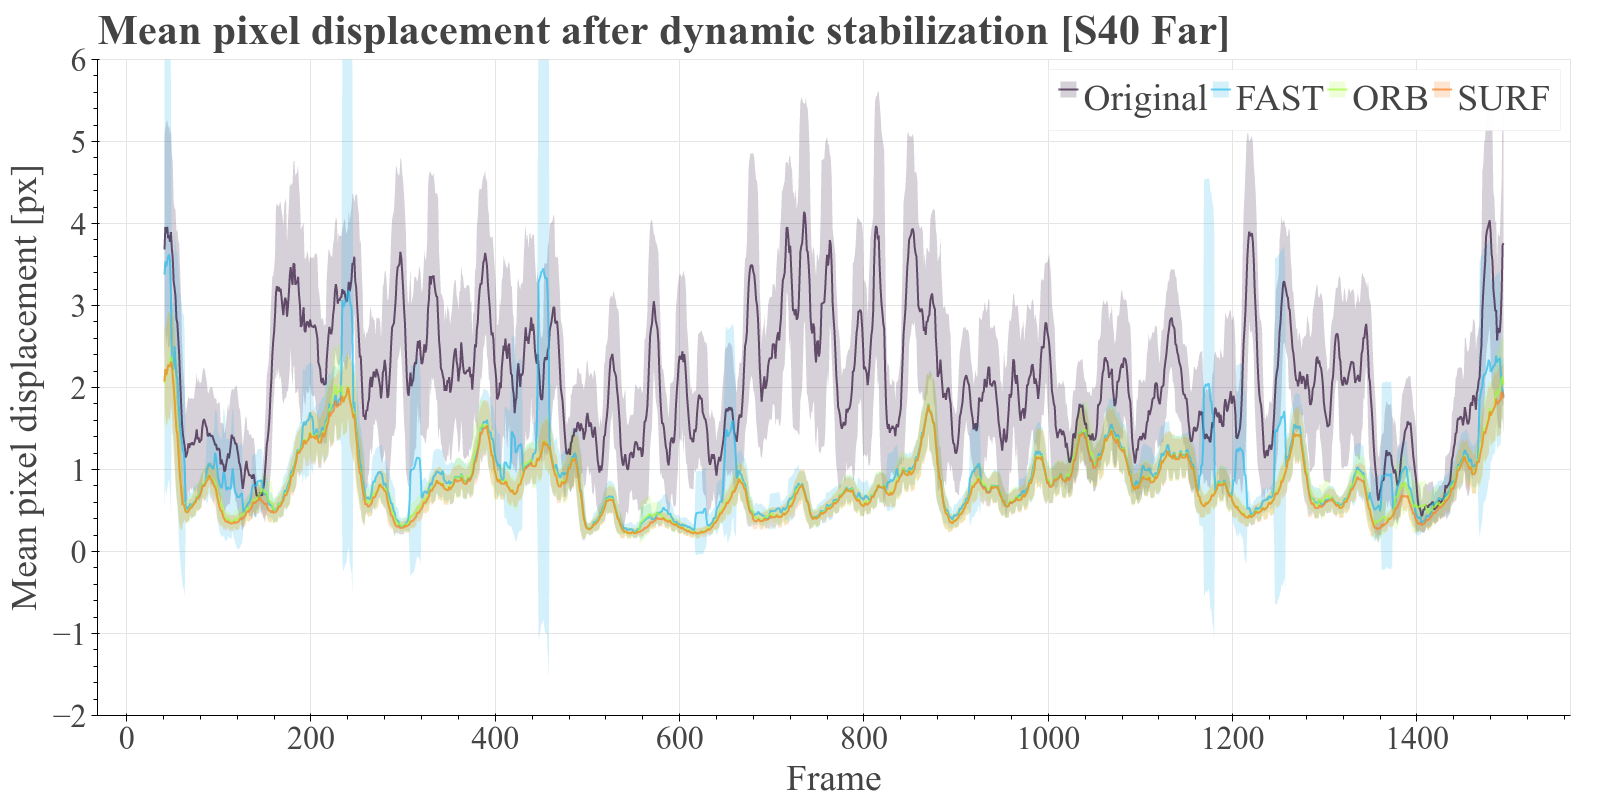
\includegraphics[width=0.5\linewidth]{diagrams/mean_pixel_shifts_after_dynamic_stabilization_s40_far.png}    &  
      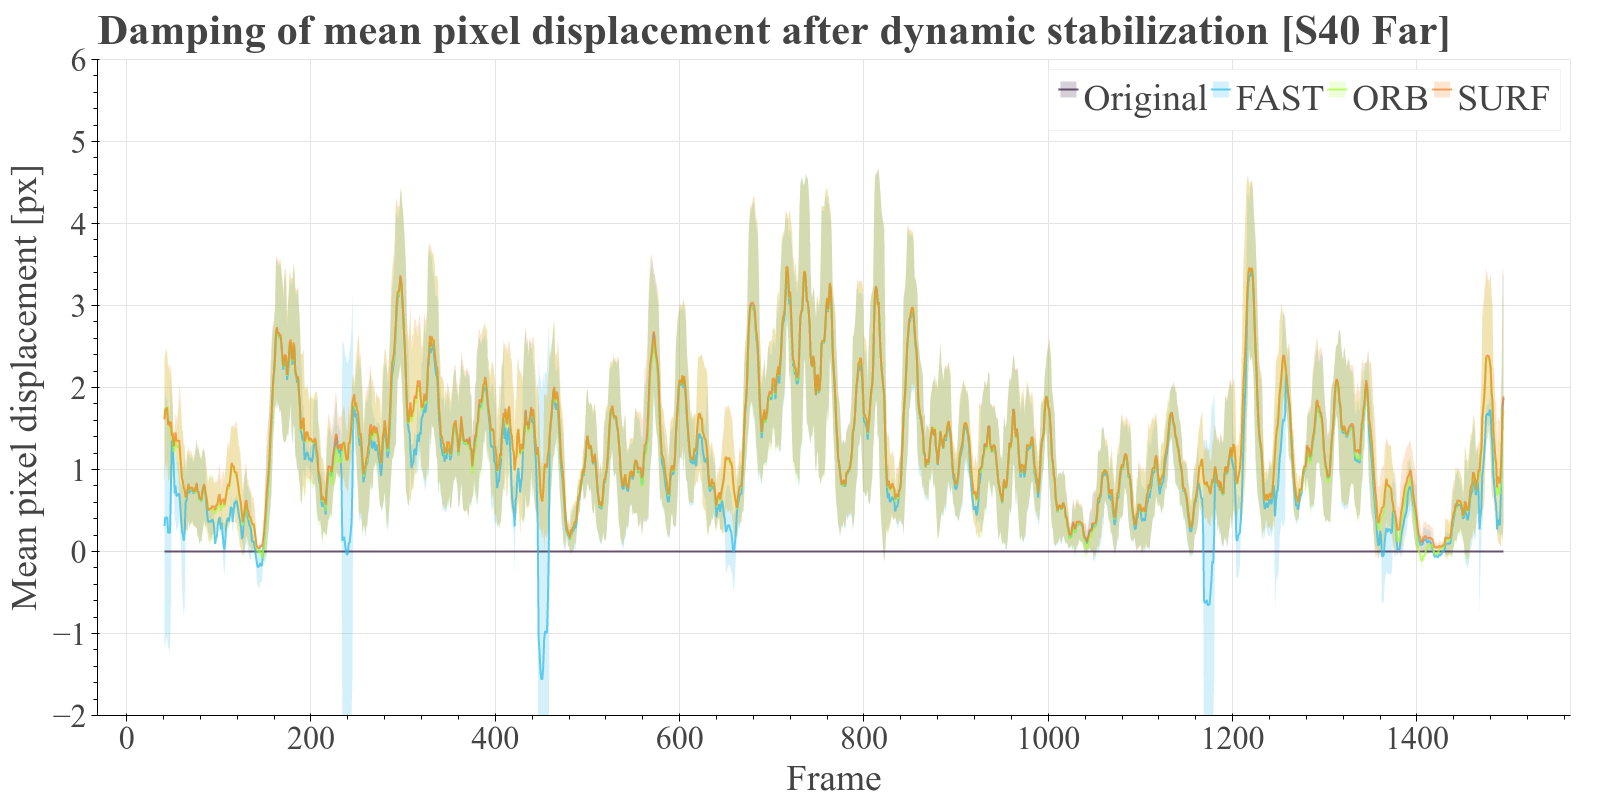
\includegraphics[width=0.5\linewidth]{diagrams/damping_mean_pixel_shifts_after_dynamic_stabilization_s40_far.png}   \\ 

      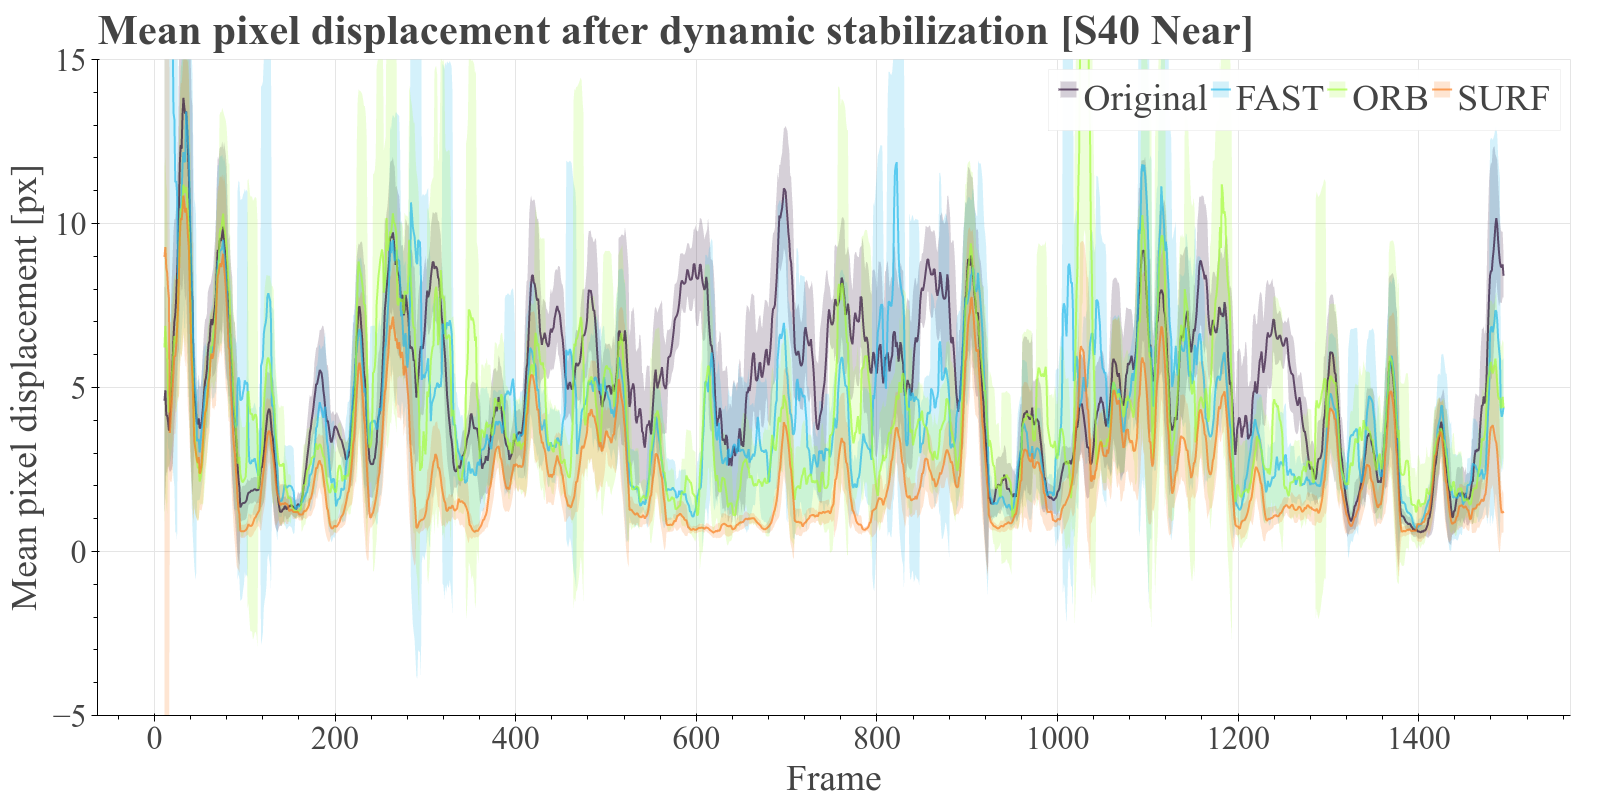
\includegraphics[width=0.5\linewidth]{diagrams/mean_pixel_shifts_after_dynamic_stabilization_s40_near.png}    &  
      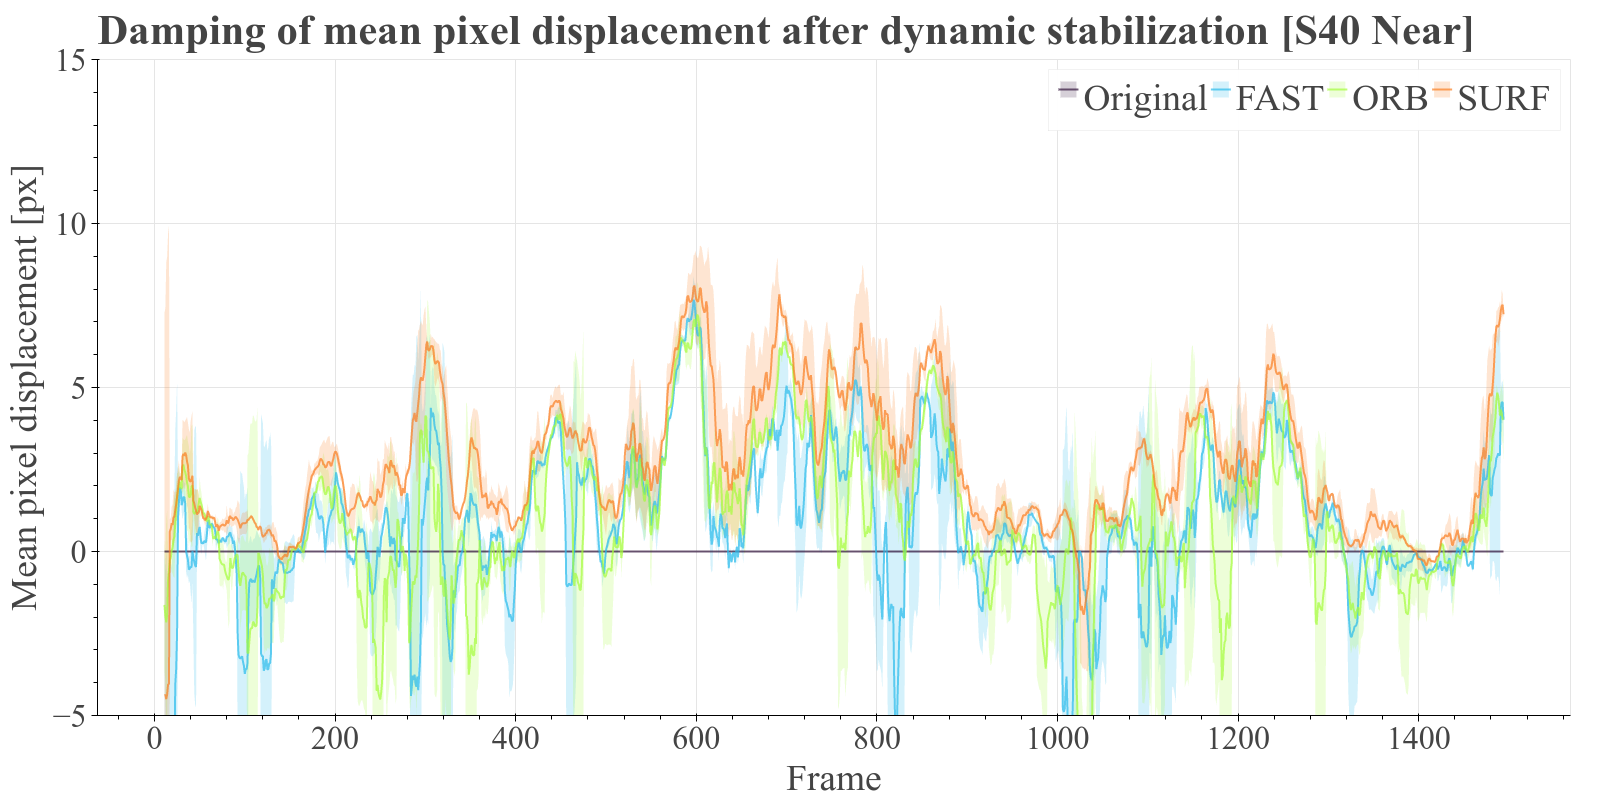
\includegraphics[width=0.5\linewidth]{diagrams/damping_mean_pixel_shifts_after_dynamic_stabilization_s40_near.png}      \\

      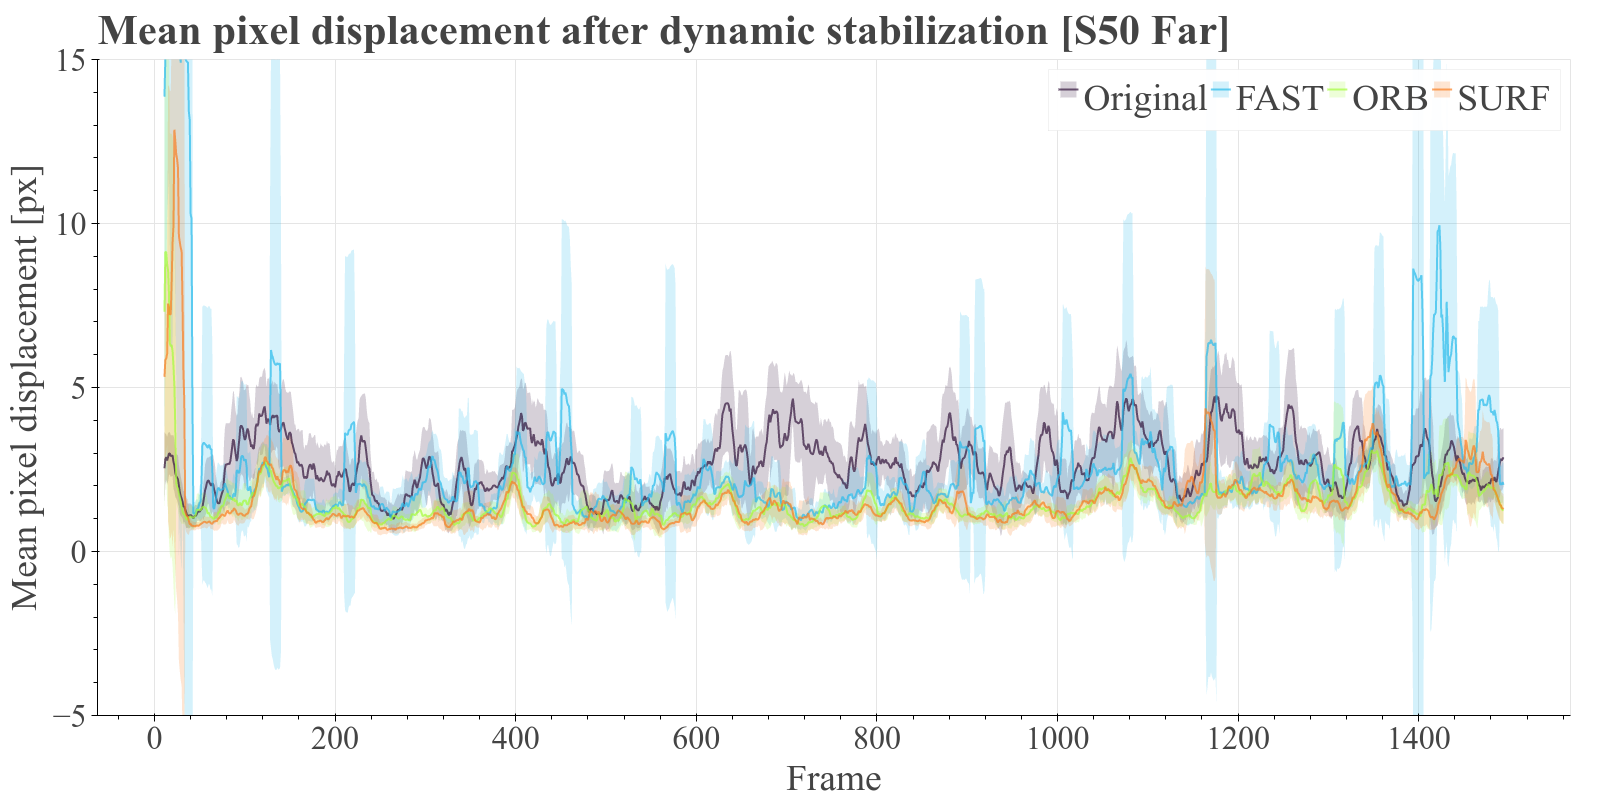
\includegraphics[width=0.5\linewidth]{diagrams/mean_pixel_shifts_after_dynamic_stabilization_s50_far.png}    &  
      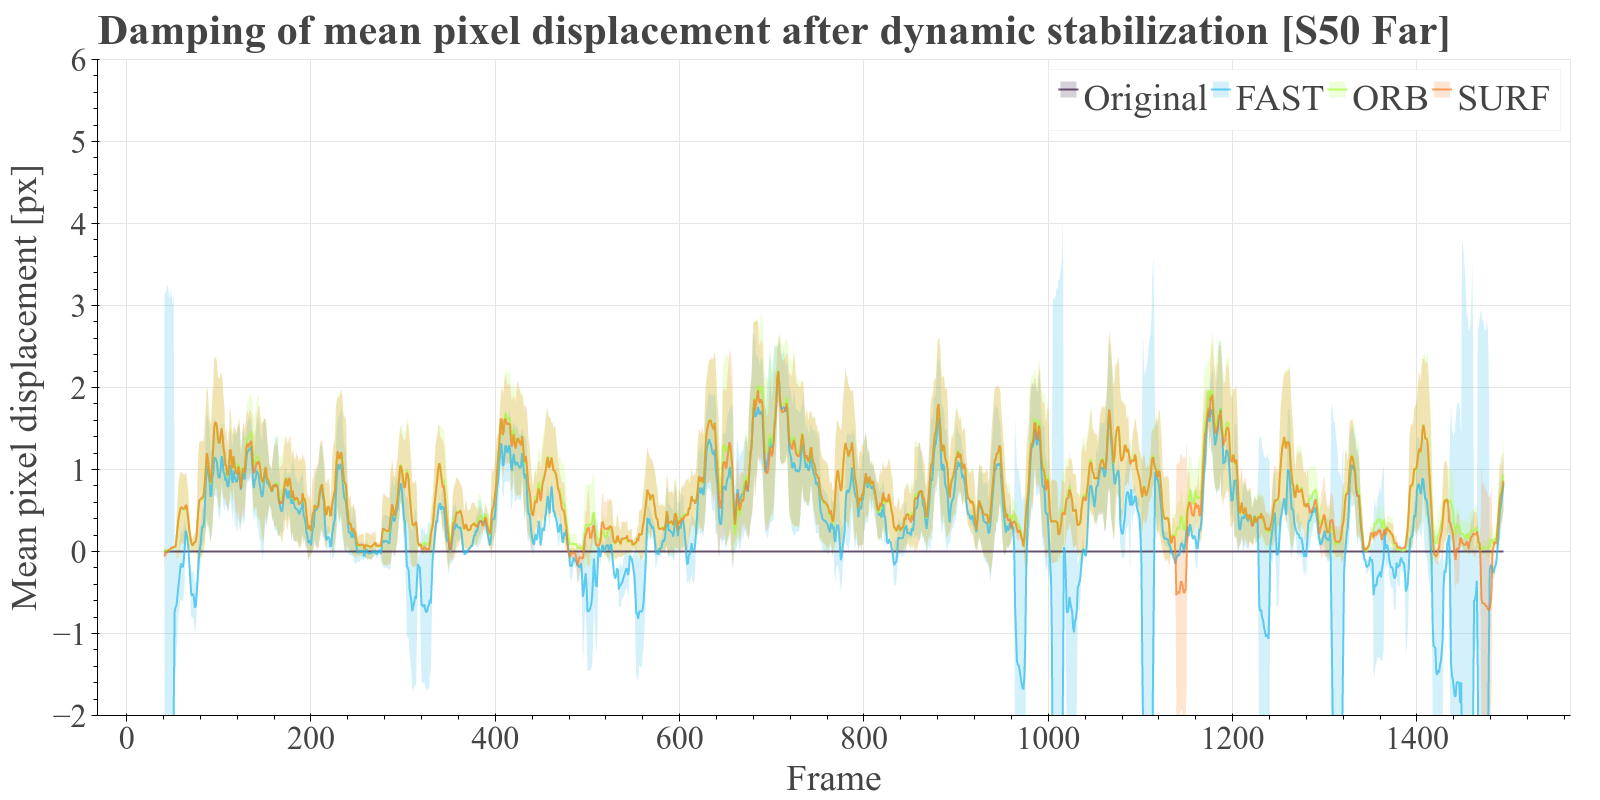
\includegraphics[width=0.5\linewidth]{diagrams/damping_mean_pixel_shifts_after_dynamic_stabilization_s50_far.png}    \\

      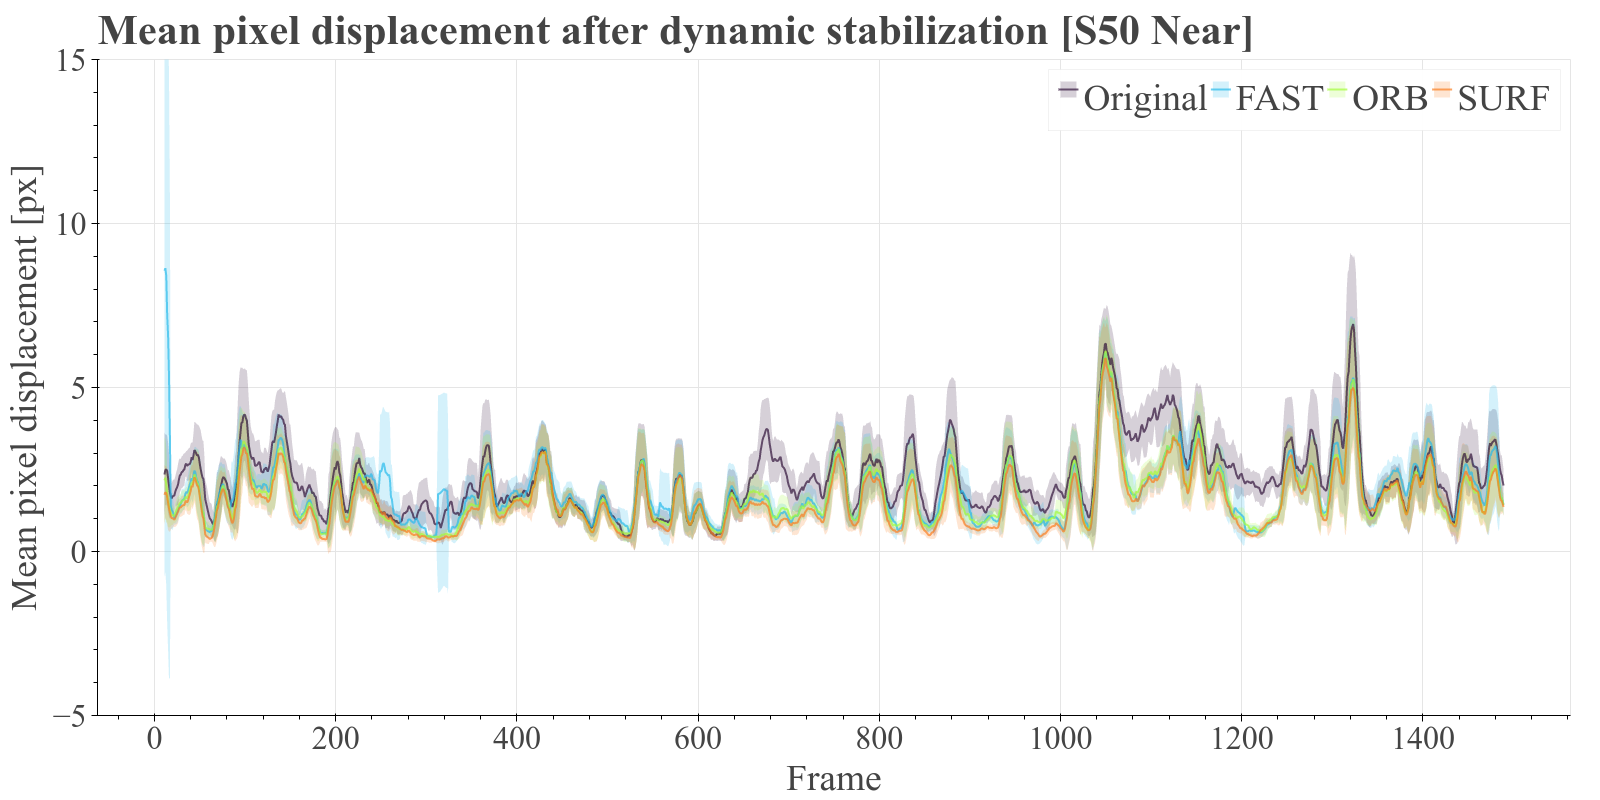
\includegraphics[width=0.5\linewidth]{diagrams/mean_pixel_shifts_after_dynamic_stabilization_s50_near.png}    &  
      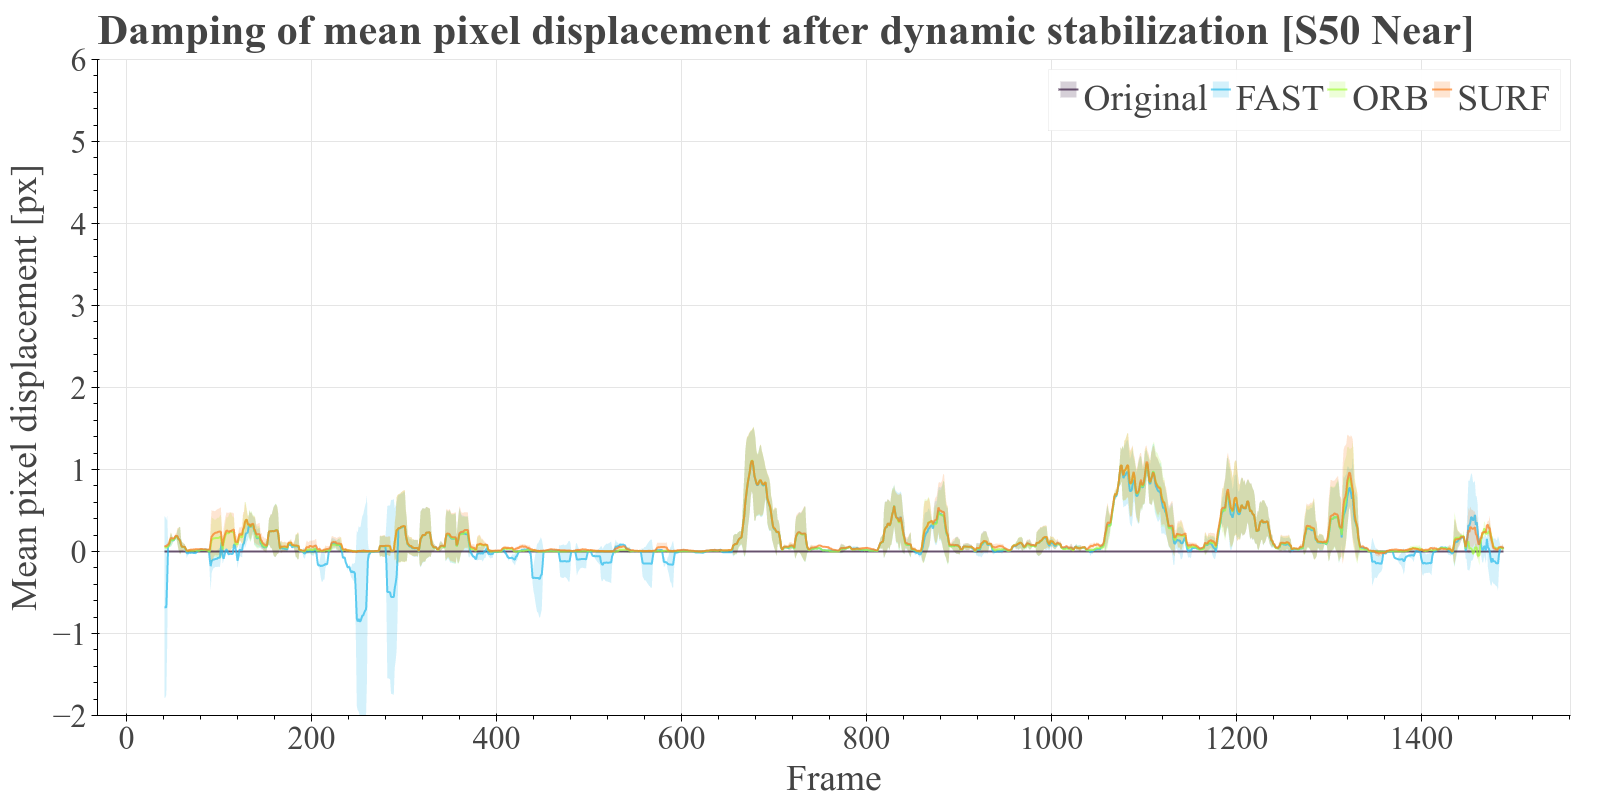
\includegraphics[width=0.5\linewidth]{diagrams/damping_mean_pixel_shifts_after_dynamic_stabilization_s50_near.png}    
    \end{tabular}
    \caption{
        Left: 
        Comparison of the three implemented dynamic stabilizers and the original not stabilized video feed using Optical Flow as metric (lower is better).
        The stabilizers are based on the 
        FAST \cite{Ghahremani_2021,opencv_library} feature detector with FREAK \cite{alahi6247715,opencv_library} feature descriptors,
        SURF \cite{bay10.1007/11744023_32,opencv_library} feature detector and
        ORB \cite{rublee6126544, opencv_library} feature detector.
        The graphs display the mean pixel shift at each frame. 
        Right: 
        The damping capabilities of the same three stabilizers (higher is better). 
        The graphs approximate the removed jitter in the mean pixel shift between the original video and the stabilizer at each frame.\\
        For visualization the values are filtered using the rolling mean over 12 frames. 
        The light areas display the standard deviation within the window.
    }
    \label{fig:dynamic_stabilization_appendix}
    \end{figure*}

    

\begin{table}[!h]
    \centering
    \begin{tabular}{ |l|l|r|r|r| } 
     \hline
     \textbf{Stabilizer} & \textbf{Camera} & \textbf{Disp.}  & \textbf{Better} & \textbf{Better [\%]} \\ 
     \hline
     Original   & \camsf{4} & 3.515 & 0     &  0.0      \\
     FAST       & \camsf{4} & 1.999 & 1279  &  85.552   \\
     ORB        & \camsf{4} & 1.632 & 1396  &  93.378   \\
     SURF       & \camsf{4} & 1.273 & 1478  &  \textbf{98.863}   \\
     \hline

     Original   & \camsn{4} & 5.084 & 0     &  0.0      \\
     FAST       & \camsn{4} & 4.371 & 983   &  65.753   \\
     ORB        & \camsn{4} & 4.222 & 1024  &  68.495   \\
     SURF       & \camsn{4} & 2.495 & 1403  &  \textbf{93.846}   \\
     \hline

     Original   & \camsf{5} & 2.624 & 0  &    0.0    \\
     FAST       & \camsf{5} & 2.749 & 983  &  65.753   \\
     ORB        & \camsf{5} & 1.510 & 1258  & 84.147    \\
     SURF       & \camsf{5} & 1.550 & 1273  & \textbf{85.151}    \\
     \hline

     Original   & \camsn{5} & 2.212 &   0   &  0.0      \\
     FAST       & \camsn{5} & 1.847 & 1028   &  68.993   \\
     ORB        & \camsn{5} & 1.671 &  1234 &    82.819 \\
     SURF       & \camsn{5} & 1.543 & 1290  &   \textbf{86.577}  \\
     \hline
    \end{tabular}
    \caption{
            Comparison of the implemented dynamic stabilizers and the original not stabilized video feed using Optical Flow as metric.
            It shows that most of the stabilizers exhibit a lower mean displacement (Disp.) after dynamic stabilization. 
            In terms of the number of frames the stabilizers all show a high number of total (Better) and relative (Better \%) frames where they have a lower mean displacement. 
            Especially for the SURF \cite{bay10.1007/11744023_32,opencv_library} feature detector (bold) the improvement is substantially.
        }
    \label{tab:dynamic_stabilization}
\end{table}